\chapter{Μελέτη της Απόδοσης του VQ H.264}
\label{chapter:chap6}

\section{Εισαγωγή}
\label{section:sect61}

\indent Σε αυτό το κεφάλαιο θα παρουσιαστούν και θα αναλυθούν τα αποτελέσματα του VQ H.264, επίσης θα γίνει σύγκριση με τις επιδόσεις του JM H.264. Επίσης θα δειχθεί ότι με την χρήση VQ μπορεί να βελτιωθεί η πολυπλοκότητα του decoder σε σχέση με αυτή του JM H.264.

\section{Encoding με VQ H.264}
\label{section:sect62}

\indent Για τις δοκιμές χρησιμοποιήθηκαν 5 βίντεο που δεν είχαν συμπεριληφθεί στο training set και τα στιγμιότυπα τους φαίνονται στο Σχήμα~\ref{fig:testvid}. To PSNR που ο VQ H.264 πέτυχε στα test video φαίνεται στον Πίνακα~\ref{table:testpsnr}. Αξίζει να σημειωθεί αποτελούν υλικό δοκιμής για το H.265 standard \cite{misc:testvid}.

\begin{table}[h!]
    \begin{center}
        \begin{tabular}{| l | l | l | l |}
        \hline
        Test Video & PSNR I (Y/U/V)dB  & PSNR P (Y/U/V)dB  & PSNR B (Y/U/V)dB       \\ \hline
        test1      & 35.15/39.72/39.67 & 41.16/43.91/43.87 & 43.00/45.14/45.22      \\ \hline
        test2      & 35.51/41.10/42.83 & 38.87/41.53/43.28 & 40.38/43.01/44.71      \\ \hline
        test3      & 30.70/39.86/41.00 & 36.68/42.64/43.76 & 38.00/43.74/44.90      \\ \hline
        test4      & 44.12/47.36/47.91 & 46.00/47.20/47.75 & 46.55/47.42/48.05      \\ \hline
        test5      & 37.01/50.12/48.70 & 44.00/49.90/49.65 & 44.78/50.46/50.29      \\ \hline
        \hline
        \end{tabular}
    \end{center}

    \caption{PSNR των Test videos με κωδικοποίηση στον VQ H.264}
    \label{table:testpsnr}
\end{table}

\begin{figure}[H]
\centering
\begin{tabular}{c c}
    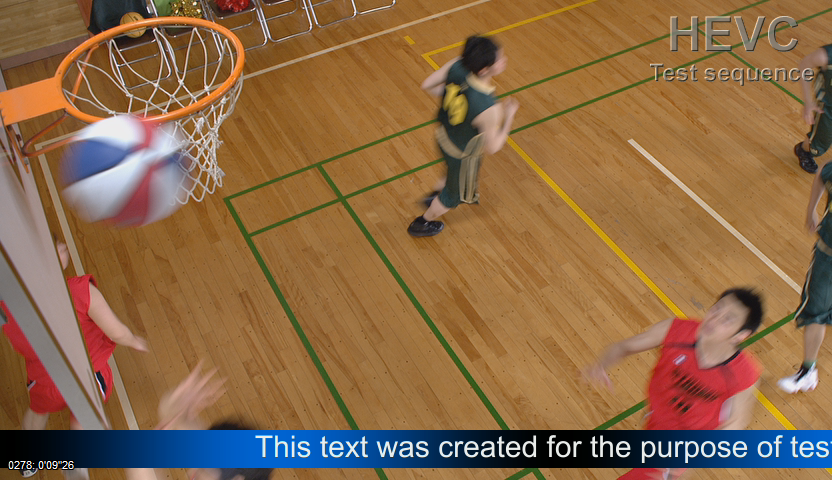
\includegraphics[height=4.0cm]{chapter6/test1.png}
    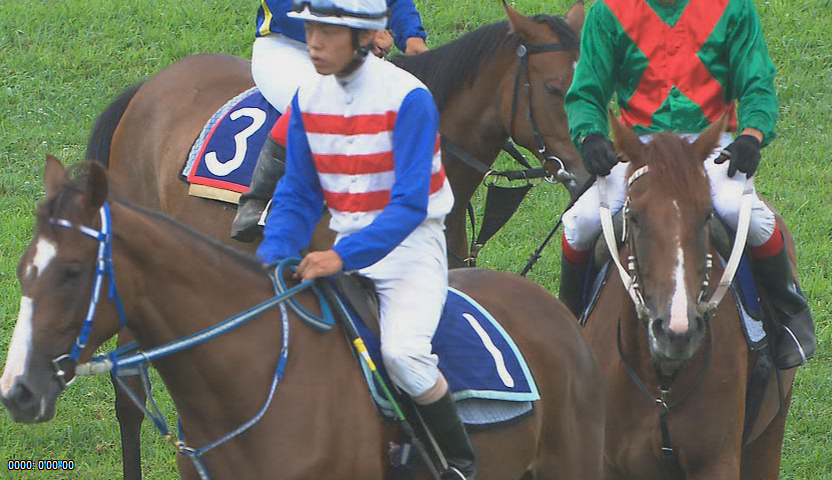
\includegraphics[height=4.0cm]{chapter6/test2.png}\\
    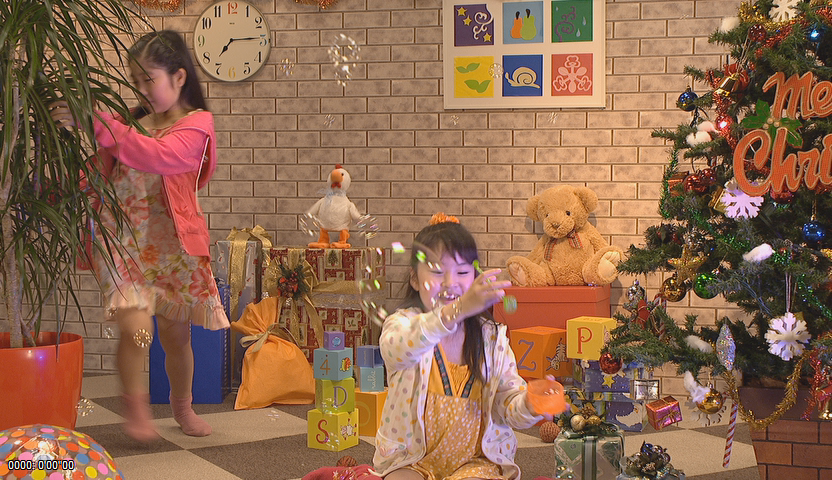
\includegraphics[height=4.0cm]{chapter6/test3.png}
    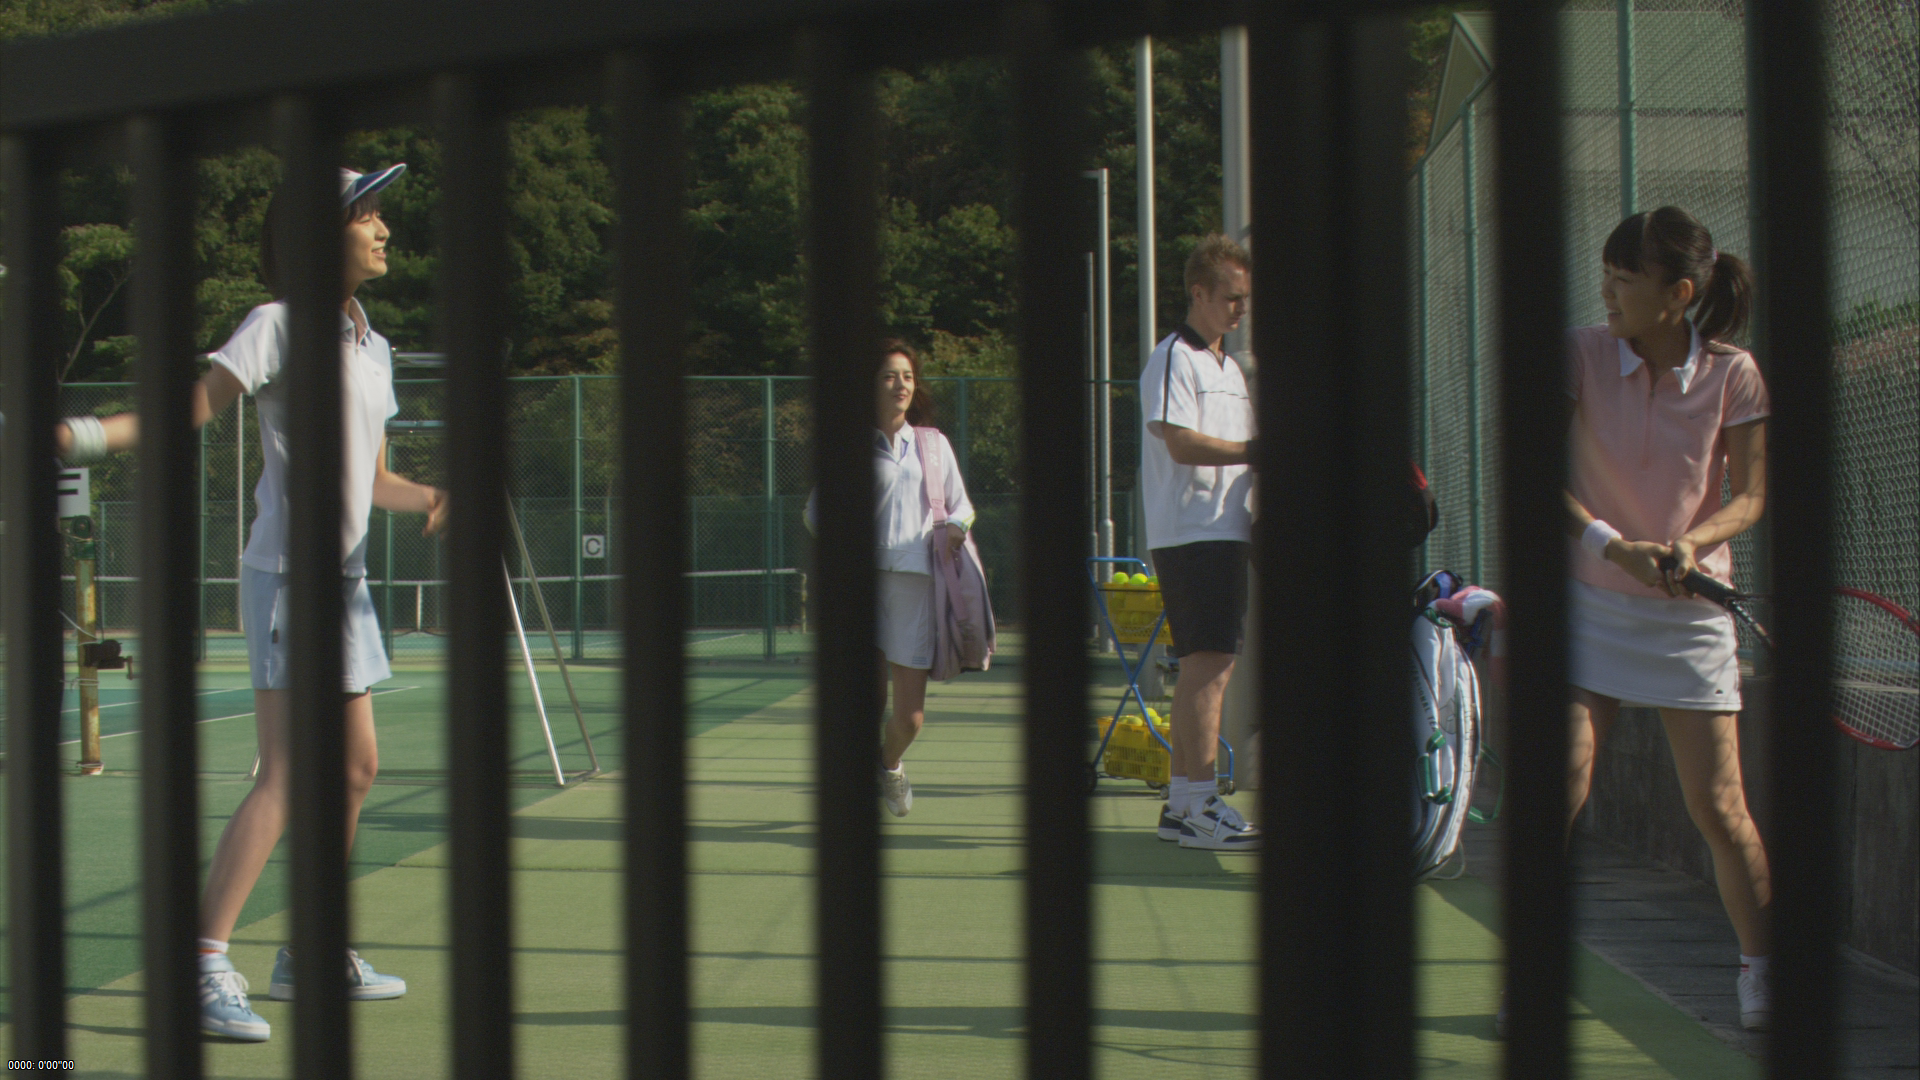
\includegraphics[height=4.0cm]{chapter6/test4.png}\\
    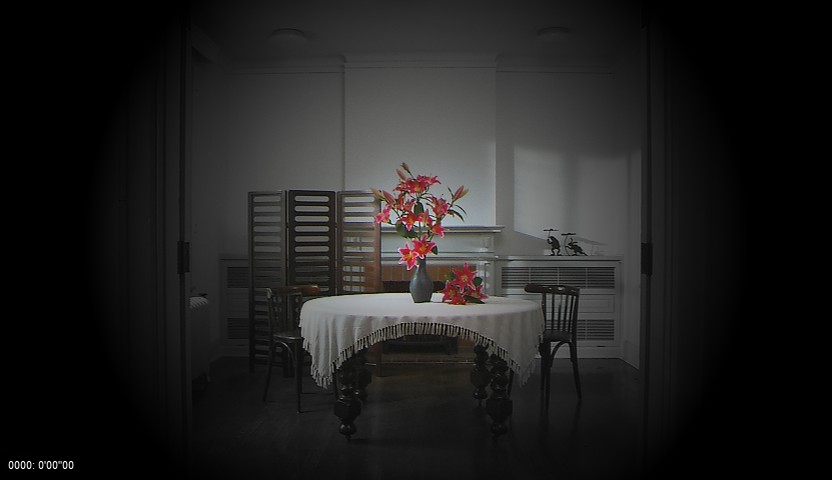
\includegraphics[height=4.0cm]{chapter6/test5.png}
\end{tabular}
\caption{Βίντεο που δοκιμάστηκαν να γίνουν encoding με τον VQ H.264.}
\label{fig:testvid}
\end{figure}

\newpage
\section{Encoding με JM H.264}
\label{section:sect62}

\indent Για να μπορούν να συγκριθούν τα αποτελέσματα των δύο encoder θα πρέπει να συμπιεστούν τα ίδια βίντεο με τον JM H.264 με τις ίδιες παραμέτρους που δεν αφορούν το VQ και προσπαθώντας να σημειωθούν τα ίδια PSNR που πέτυχε και ο VQ H.264. Αυτό πραγματοποιήθηκε δοκιμάζοντας διάφορα QP για τα καρέ I,P,B. Επειδή στον VQ H.264 παρατηρείται ότι το U,V αποδίδει πολύ καλύτερα από το Υ σε κάποια βίντεο χρειάστηκε να υπολογιστεί ο βεβαρημένος μέσος όρος $avg = 0.66*PSNRY+0.16*PSNRU+0.16*PSNRV$ έτσι ώστε να ισχύει $avg_{vq}=avg_{jm}$. Τα αποτελέσματα φαίνονται στον Πίνακα~\ref{table:jm264}.
Η ποσοστιαία διαφορά ως προς τον JM φαίνεται στον Πίνακα~\ref{table:jmvqdiff} και θα μπορούσε να χαρακτηριστεί πολύ μικρή κάτι το οποίο καθιστά την μεταξύ τους σύγκριση δίκαια.

\begin{table}[h!]
    \begin{center}
        \begin{tabular}{| l | l | l | l |}
        \hline
        Test Video & PSNR I (Y/U/V)dB  & PSNR P (Y/U/V)dB  & PSNR B (Y/U/V)dB       \\ \hline
        test1      & 36.31/38.88/38.90 & 42.01/43.95/44.54 & 43.50/44.75/45.49      \\ \hline
        test2      & 37.31/38.43/40.00 & 40.50/41.14/42.24 & 40.50/41.45/42.54      \\ \hline
        test3      & 33.94/37.24/37.85 & 38.64/40.75/41.45 & 38.45/40.51/41.25      \\ \hline
        test4      & 45.18/46.83/47.86 & 45.75/47.13/48.18 & 46.10/47.29/48.21      \\ \hline
        test5      & 39.20/46.76/47.34 & 43.94/47.66/48.28 & 45.14/49.29/49.76      \\ \hline
        \hline
        \end{tabular}
    \end{center}

    \caption{PSNR των Test videos με κωδικοποίηση στον JM H.264}
    \label{table:jm264}
\end{table}

\begin{table}[h!]
    \begin{center}
        \begin{tabular}{| l | l | l | l |}
        \hline
        Test Video & \% Diff I  & \% Diff P & \% Diff B   \\ \hline
        test1      & 1,40	    & -1,40	    & -0,93       \\ \hline
        test2      & 0,83	    & -5,11	    & -4,23       \\ \hline
        test3      & 3,53	    & -5,21	    & -5,49       \\ \hline
        test4      & 1,35	    & -0,87	    & -0,18       \\ \hline
        test5      & 1,69	    & -5,38	    & -2,76       \\ \hline
        \hline
        \end{tabular}
    \end{center}

    \caption{Διαφορές του PSNR JM-VQ. Στα θετικά πρόσημα ο JM είναι καλύτερος από τον VQ ενώ στα αρνητικά πρόσημα  το ανάποδο.}
    \label{table:jmvqdiff}
\end{table}

\newpage
\section{Αποτελέσματα των VQ H.264,JM H.264}
\label{section:sect63}

\indent Για να γίνει η σύγκριση θα υπολογιστούν τα συνολικά bits που ο JM H.264 χρειάστηκε για να αποθηκεύσει τους κβαντοποιημένους συντελεστές του μετασχηματισμού. Αυτή η πληροφορία μας παρέχεται απευθείας από την έξοδο του encoder. Αυτό γίνεται γιατί ουσιωδώς τα $VQ_{indices}$ αντιστοιχούν μόνο στην πληροφορία που  παρέχουν τα residuals, όπως και οι συντελεστές του μετασχηματισμού. Ως γνωστόν στα standard συμπίεσης βίντεο όπως το H.264 αλλά και στα mpeg1,2,4 η διαδικασία της κβαντοποίησης οδηγεί μόνο σε μηδενικούς συντελεστές, κατά συνέπεια το συγκεκριμένο block δεν κωδικοποιείται και η παρουσία σηματοδοτείται με κάποιο συγκεκριμένο flag (CBP) στο .264 αρχείο. Στην περίπτωση που όλο το macroblock αποτελείται από μηδενικά block τότε δεν κωδικοποιείται καθόλου. Στο επόμενο βήμα υπολογίστηκε ο αριθμός των Skipped macroblock και αφαιρέθηκαν 16 Υ vectors και 8 UV vectors για κάθε macroblock. Στο επόμενο βήμα πολλαπλασιάζεται η εντροπία είτε του Πίνακα~\ref{table:conentropy} (με την χρήση context) είτε του Πίνακα~\ref{fig:trainingset} (χωρίς την χρήση context) με την διάσταση του VQ για να υπολογιστεί πόσα bits χρειάζονται για κάθε block $dxd$. Τέλος πολλαπλασιάζονται τα bits που χρειάζονται ανά block με τον αριθμό των non-skipped blocks και έτσι εκτιμάται το μεγέθος που θα χρειάζονταν για την κωδικοποίηση των $VQ_{indices}$ μετά απο συμπίεσης. Αναμένεται μετά από χρήση είτε πινάκων Huffman είτε με την χρήση CABAC, να σημειωθούν τα αποτελέσματα τα οποία φαίνονται στο Σχήμα~\ref{fig:compare1}.

\begin{figure}[H]
    \centering
    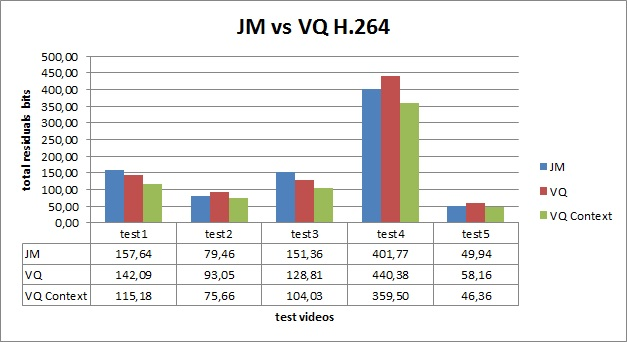
\includegraphics[width=0.8\textwidth]{chapter6/compare1.jpg}
    \caption{Σύγκριση των bits του JM H.264 και VQ H.264 με context entropy και χωρίς context.}
    \label{fig:compare1}
\end{figure}

\indent Εκτός από την σύγκριση της αποδοτικότητας της συμπίεσης έγινε προσπάθεια να συγκριθούν και οι χρόνοι κωδικοποίησης και αποκωδικοποίησης. Όπως αναφέρθηκε ο VQ Η.264 κάνει όλη την άχρηστη για αυτόν δουλειά του μετασχηματισμού, κβαντοποίησης, αντίστροφου μετασχηματισμού, αντίστροφης κβαντοποίησης. Συνεπώς, χρησιμοποιήθηκε το Intel VTune για να βρεθεί ο χρόνος αυτόν των συναρτήσεων και να αφαιρεθούν από τον συνολικό. Έτσι έγινε μια καλή προσέγγιση των επιδόσεων του VQ H.264 και η σύγκρισή με τον JM H.264 φαίνεται στο Σχήμα~\ref{fig:compare2} και στο Σχήμα~\ref{fig:compare3}. Παρατηρείται ότι στον VQ H.264 encoder υπάρχει αύξηση της πολυπλοκότητας το οποίο οφείλεται αποκλειστικά στην αναζήτηση FastNN. Στον VQ H.264 decoder παρατηρείται μια αναίσθητη διαφορά.

 \begin{figure}[H]
    \centering
    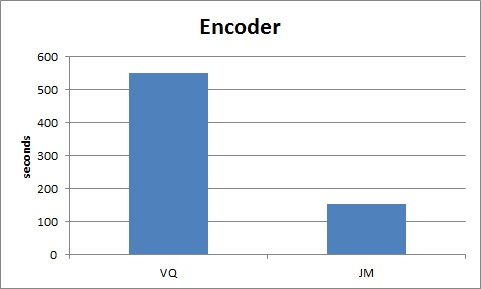
\includegraphics[width=0.8\textwidth]{chapter6/compare2.jpg}
    \caption{Σύγκριση του χρόνου εκτέλεσης των encoder JM H.264 και VQ H.264.}
    \label{fig:compare2}
\end{figure}

 \begin{figure}[H]
    \centering
    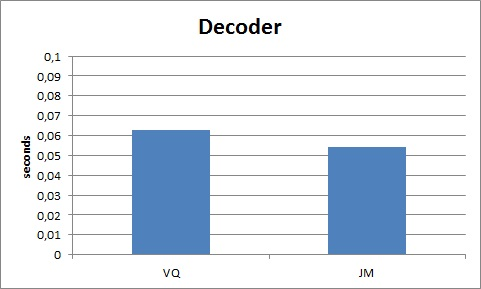
\includegraphics[width=0.8\textwidth]{chapter6/compare3.jpg}
    \caption{Σύγκριση του χρόνου εκτέλεσης των decoder JM H.264 και VQ H.264.}
    \label{fig:compare3}
\end{figure} 